\chapter{PN and orthogonal sequences}

There are two main goals need to be pursued for receiving higher localization accuracy.\\    
First the code which is used for the under water localization needs its auto-correlation approaching a Dirac impulse. Thus one get advantageous detection capabilities.\\
The next factor are cross-correlation properties, which should meet certain criteria for improving the separation from other sequences. These will come in handy if noise, reflections and other artifacts emerge.

\section{Pseudo-random codes}

There are a couple of principles to generate PN sequences. Most of these methods use linear feedback shift registers to generate the codes by an initial condition. In this project I will concertize my research on gold codes, Kasami-Codes and the classical m-sequences which are also used for generating gold codes.\\
M-sequences are binary PN codes, which are generated by linear shift registers with feedback. The sequences are periodic and contain the same number of zeros and ones \cite{proakis08}. 
M-sequences need to fulfill certain criteria.  First its length is defined by $N=2^n - 1$ where $n$ is the maximum degree of the generator polynomial $f(X)$ \cite{sarwate80}.
 \begin{equation}
	I.~~~ \lvert u\rvert=2^n-1=N,~~~\text{from polynomial}~~h(x) \text{of degree}~~n
\end{equation}
\begin{equation}
	II.~~~\dfrac{N}{gcd(N,q)=N},~~~\text{from decimation polynomials}~~\widetilde{h(x)}
\end{equation}
Second the cross-correlation between m-sequences needs to take three values only, which are $-1$, $-t(n)$, $t(n) - 2$. With it $t(n)$ is defined by $1+2^{\lfloor0.5(n+2)\rfloor}$ \cite{sarwate80}.
If every pair of m-sequences is a preferred pair, they form a maximal connected set and these sets have a limited cardinality. Experiments from Gold and Koptizke showed that the number of such connected pairs is limited. Between degrees $$$$ \cite{gold65}. To get an m-sequence we need a primitive which needs to fulfill certain citeria. 


\fignoframe{images/lfsr}{Basic structure of an LFSR (Linear Feedback Register). \cite{proakis08}}{fig:framelessFigures}

\subsection{Gold Codes}

Because of not optimal cross-correlation properties m-sequences alone are not applicable for the project. But if these type of codes are combined their correlation qualities can change. Gold Codes are m-sequences where two of them with same length are modulo-2 summed. \cite{proakis08} \\
The gold code which has the highest similarity to Gaussian random variable has a degree of 13. Thus, a generator polynomial pair of $x^13+x^4+x^3+x+1$ and $x^13+x^12+x^10+x^9+x^7+x^6+x^5+x+1$ is chosen \cite{merrifield} . (@TODO: remove this example)


\begin{equation}
Gold(u,v)=\{u,v,u\oplus v,u\oplus(v \ll1),\dots,u\oplus(v\ll N-1)\}
\end{equation}

\fignoframe{images/gold}{LFSR structure of preferred generator polynom of degree 13). \cite{merrifield}}{fig:framelessFigures}

\subsection{Kasami Codes}

Kasami sequences are constructed in the same fashion by using m-sequences with the exception that a second sequence, which is used in the modulo sum, is formed by decimating the default m-sequence by  $2^{m/2}$ \cite{proakis08} \cite{sarwate80} \cite{peterson72}. 

\begin{equation}
w=u[2^{N/2}+1]=\{u_1,\dots, u_i, \dots,u_{N}|\text{take every }i\text{-th bit of u}\} 
\end{equation}
\begin{equation}
Kasami(u)=\{u,u\oplus w,u\oplus(w \ll1),\dots,u\oplus(w\ll2^{N/2}-2)\}
\end{equation}


\section{Comparison}

For the localization process by orthogonal codes certain criteria needs to be met, which were named in the first chapter. To compare the before explained code types three measures are introduced. \\ 
The first one is the peak to side-lobe ratio (PSR) \ref{eq:psr}. This measure is defined by subtracting the mean from the peak of the auto-correlation. Then this value get divided by the standard deviation of the same auto-correlation. A higher PSR value signifies a smaller error between the auto correlation and the perfect Dirac rsulting in better detection capability. The second one is the ratio between the auto-correlation peak and the maximum of the cross-correlation (ACR) \ref{eq:acr}. Here a higher value indicates good code separation qualities. The last one is the correlation coefficient showing if there are similar anchros \ref{eq:coeff}, which would be a bad indicator.

\begin{equation}
PSR=\dfrac{max\{x_{ac}\}-\overline{x_{ac}}}{\sigma_{ac}}
\label{eq:psr}
\end{equation}

\begin{equation}
ACR=\dfrac{max\{x_{ac}\}}{max\{{x_{cc}\}}}
\label{eq:acr}
\end{equation}

\begin{equation}
\rho(a1,a2)=\dfrac{cov\{a1,a2\}}{\sigma_{a1}\cdot\sigma_{a2}}
\label{eq:coeff}
\end{equation}
\begin{figure}[h]
	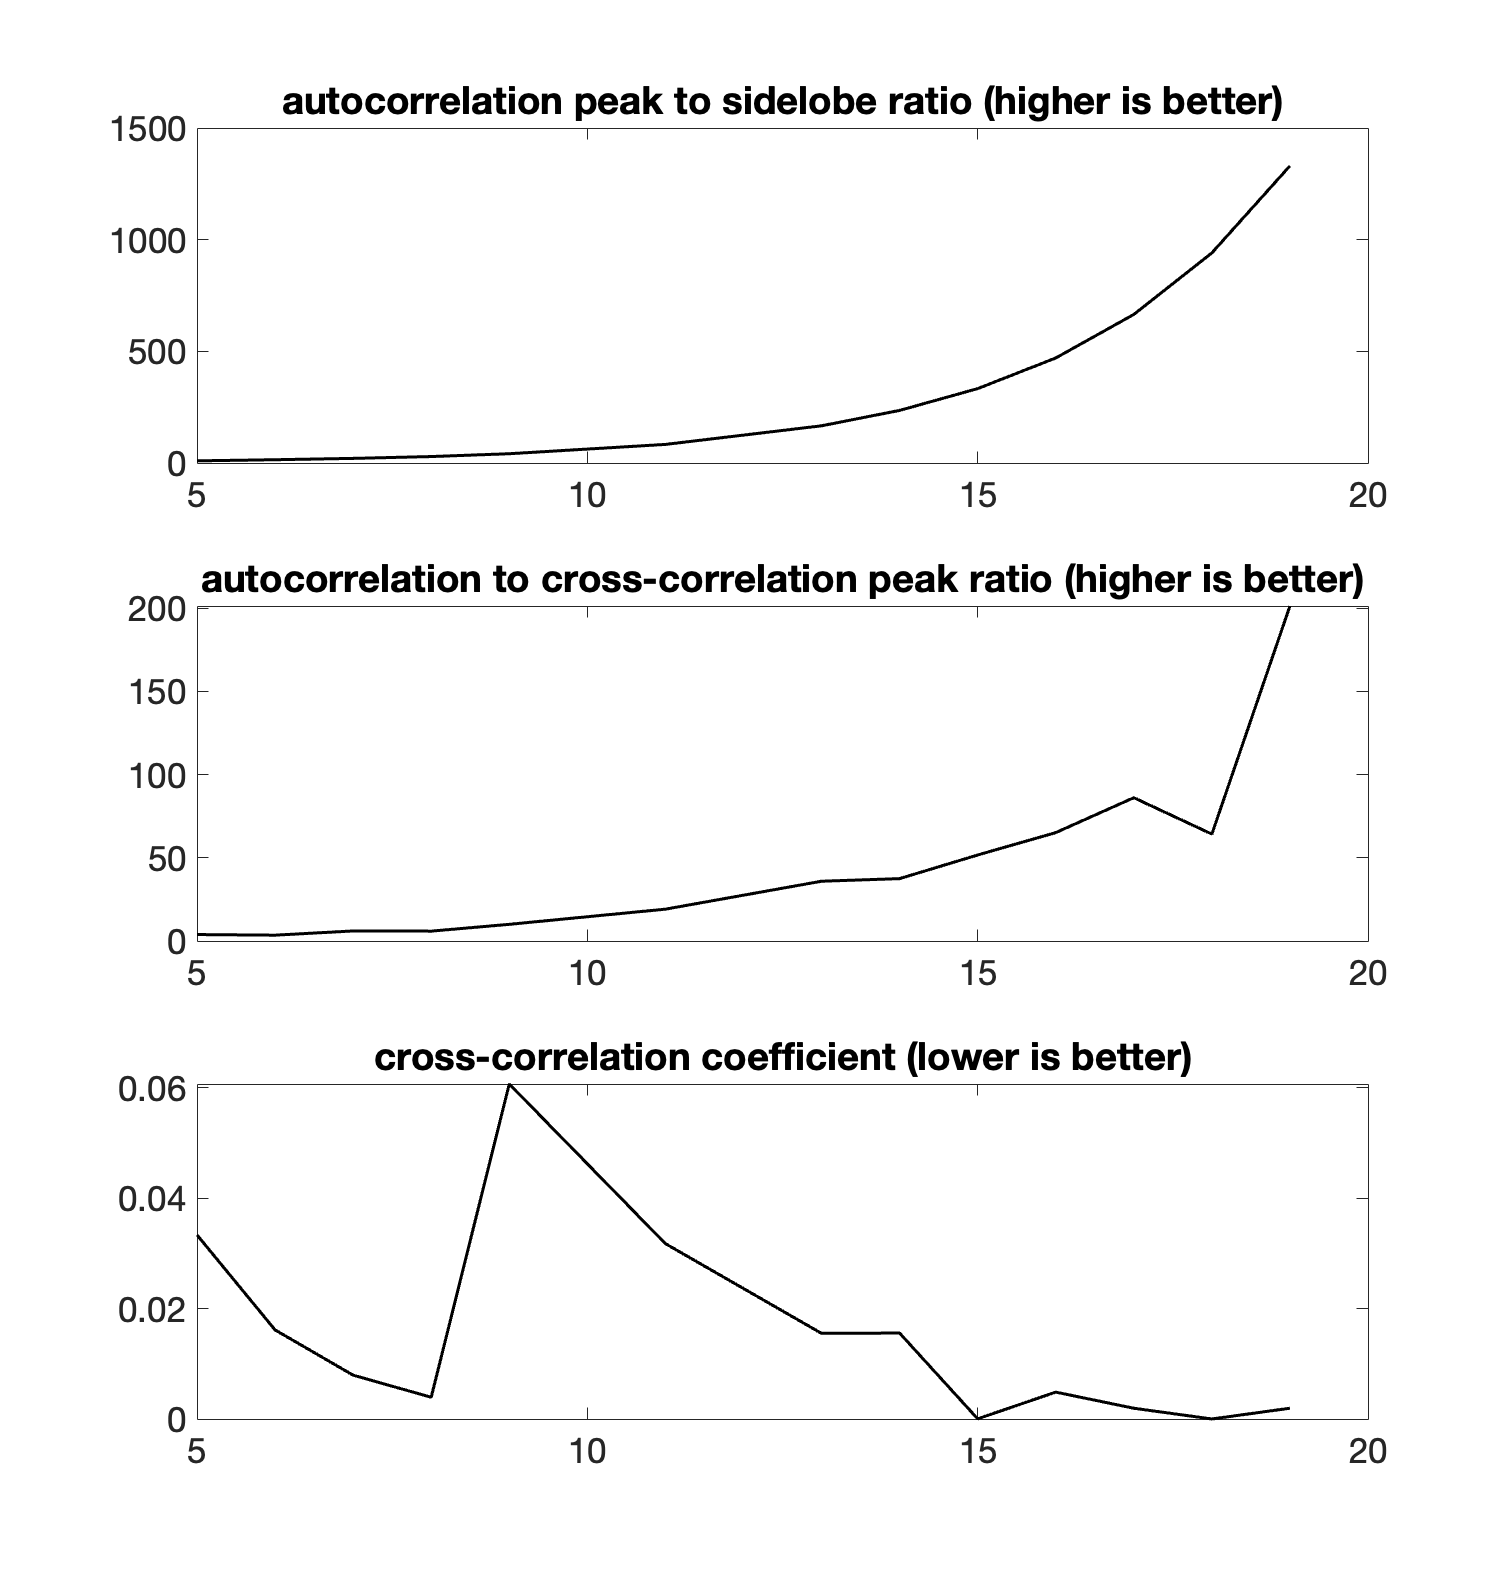
\includegraphics[width=8cm]{images/matlabplots/mseq}

	\caption{Maximum Length Sequence evaluation}
\end{figure}

\begin{figure}[h]
	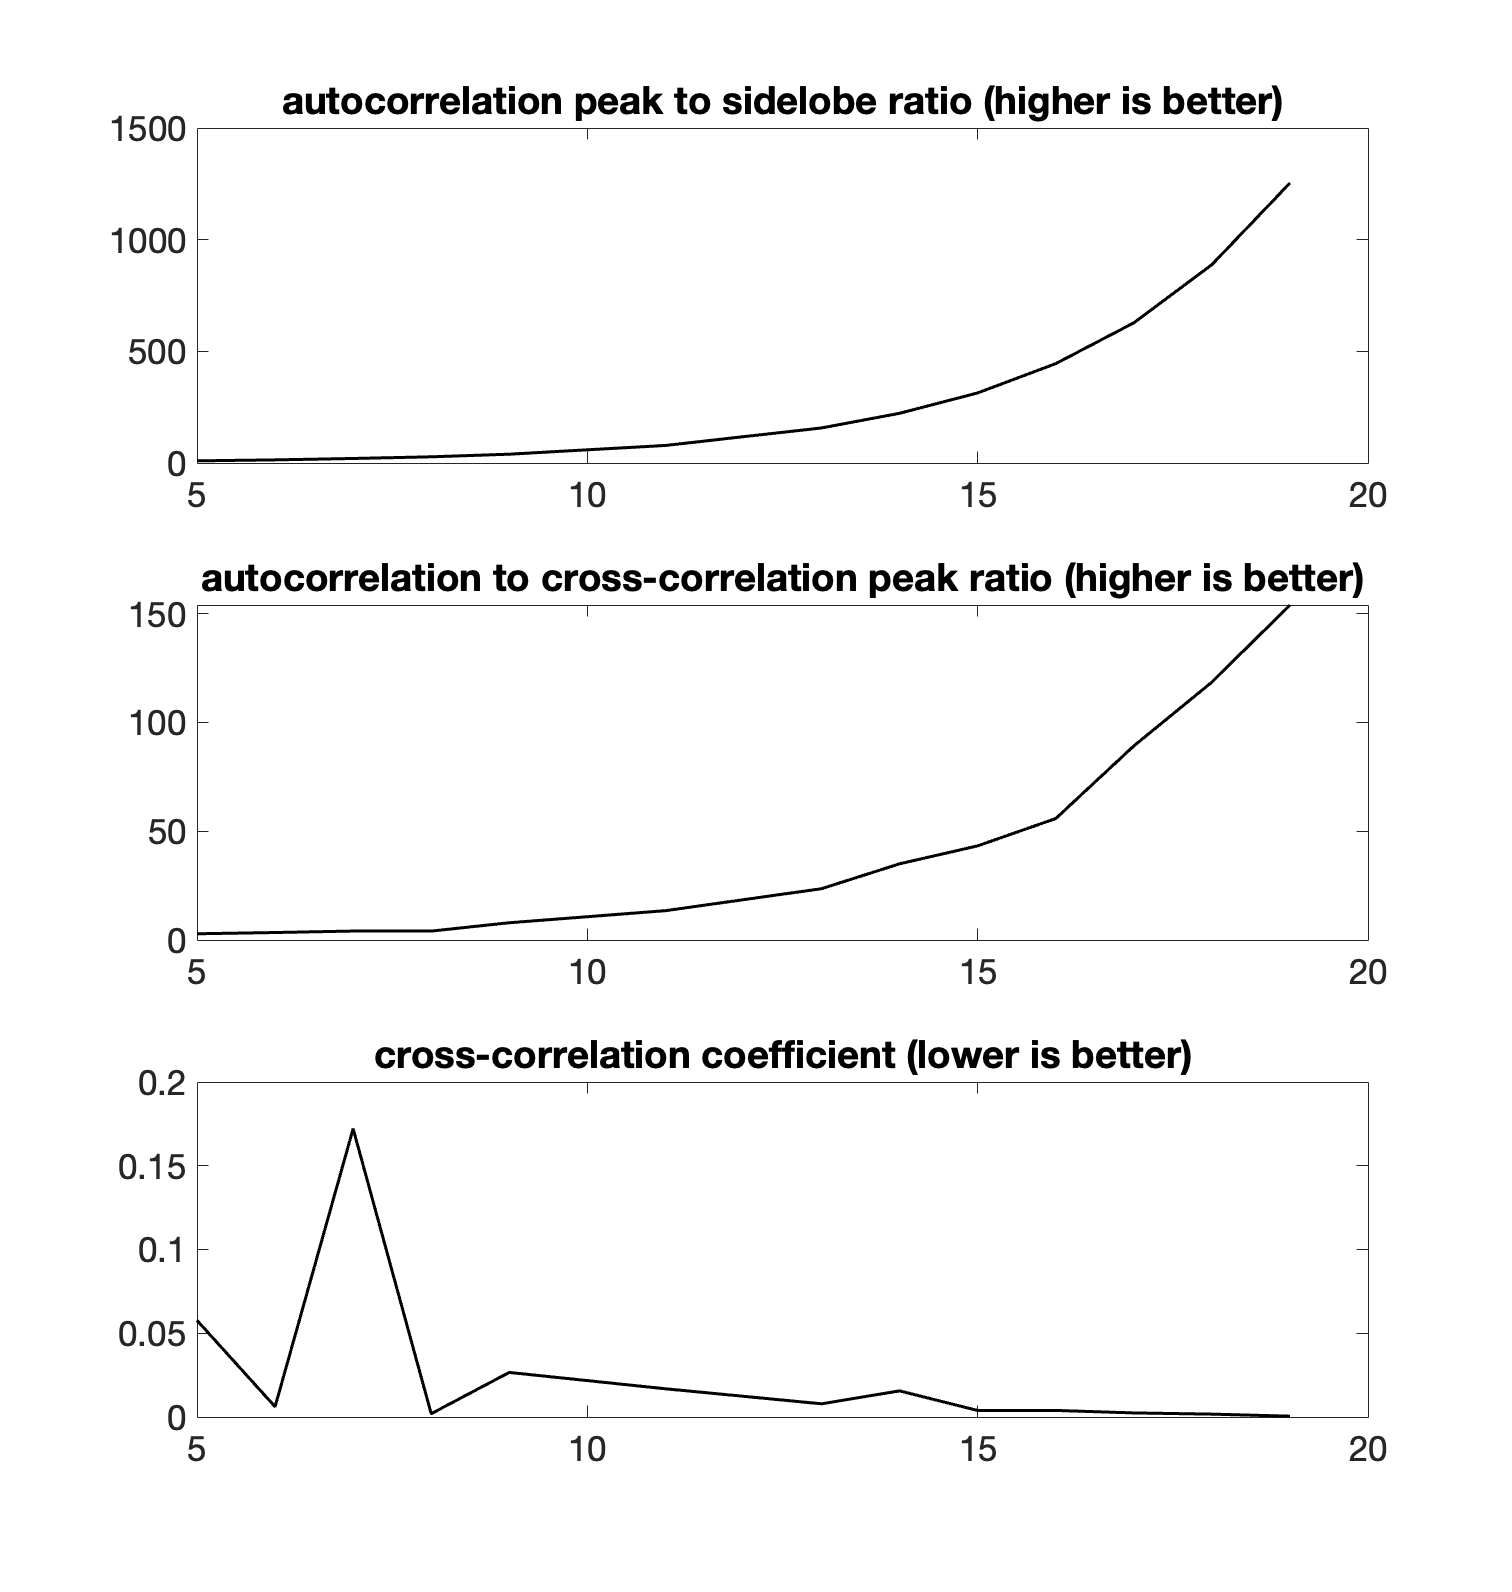
\includegraphics[width=8cm]{images/matlabplots/gold}

	\caption{Gold sequence evaluation}
\end{figure}

\begin{figure}[h]
	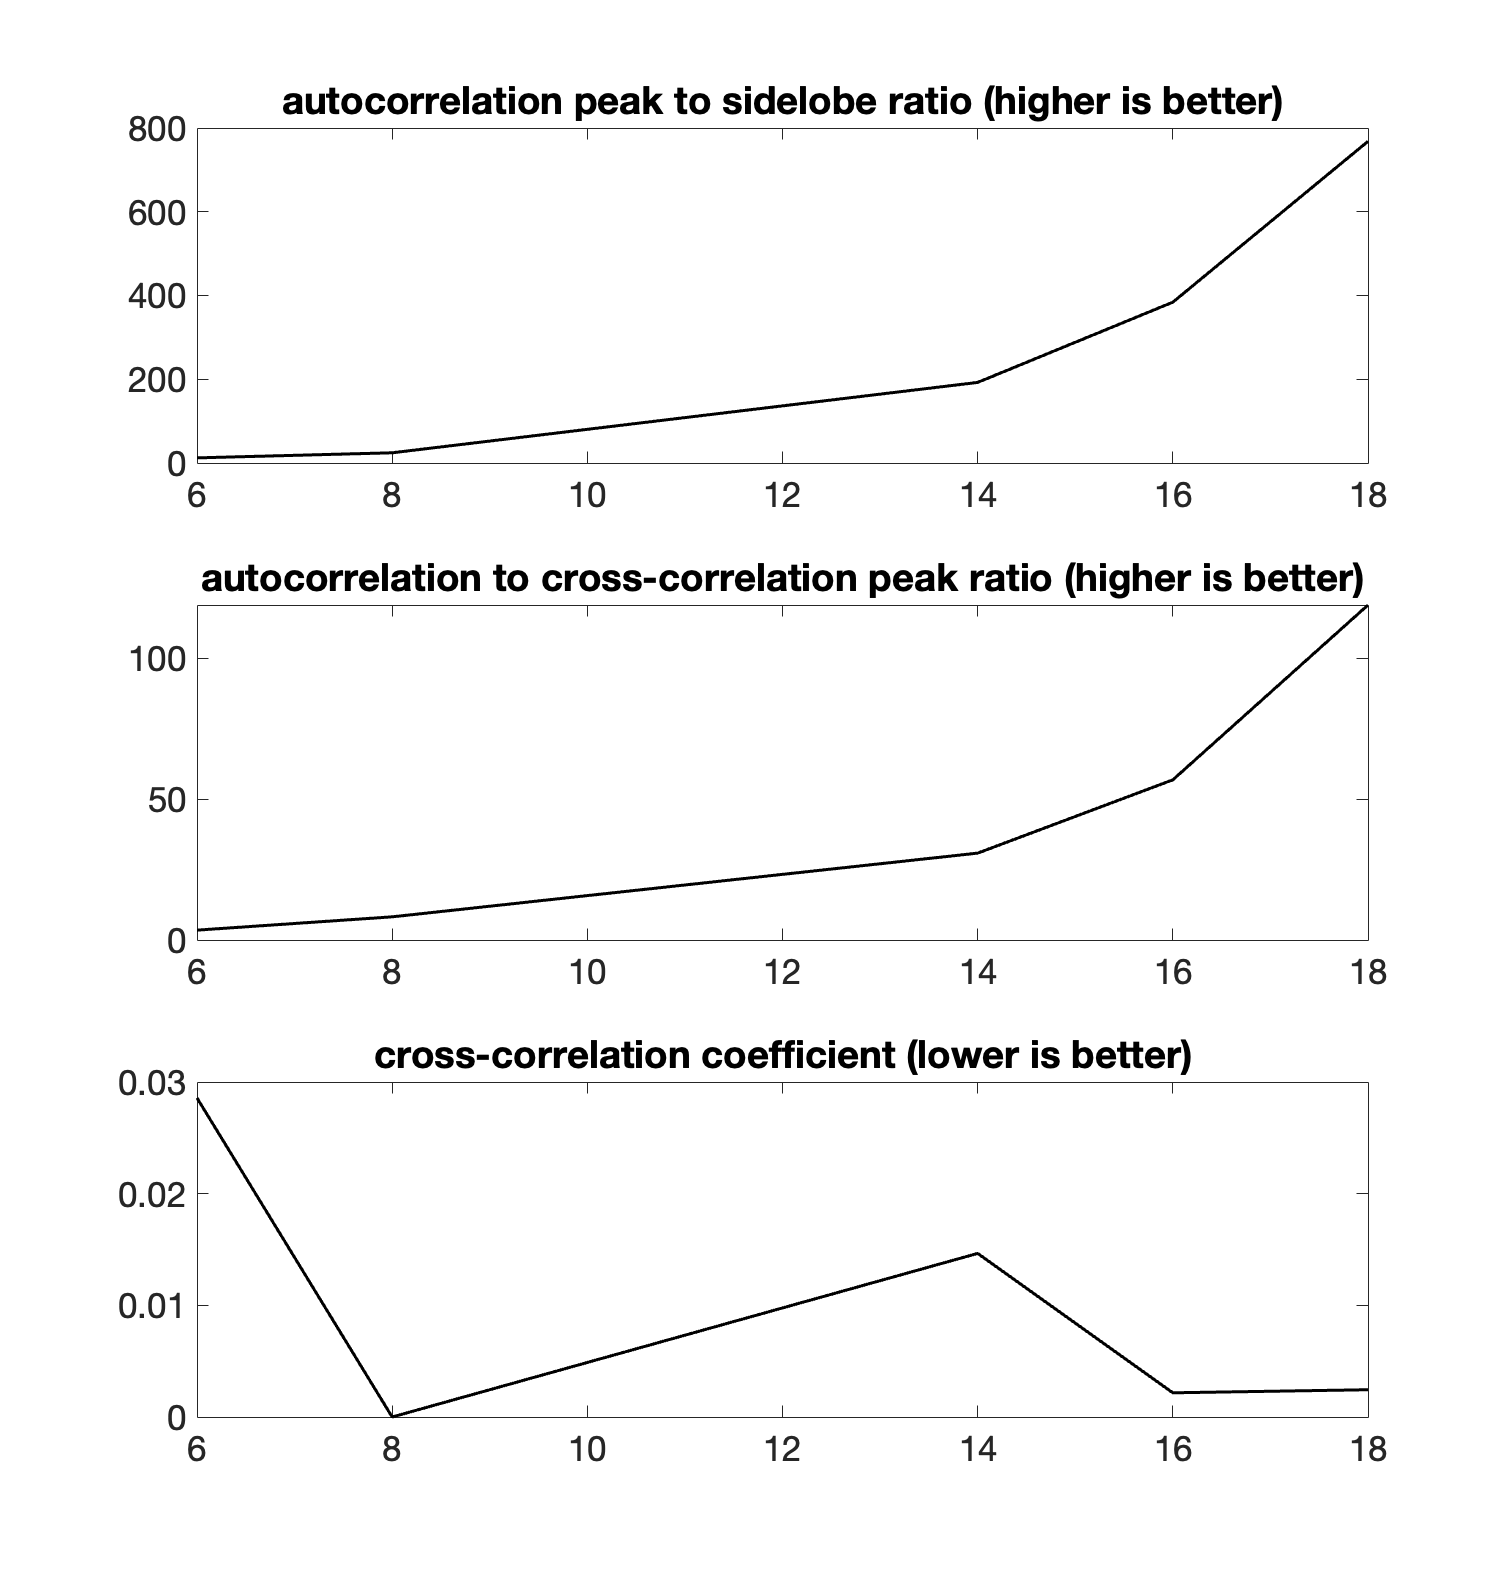
\includegraphics[width=8cm]{images/matlabplots/kasami}

	\caption{Kasami sequence evaluation}
\end{figure}
%\fignoframe{images/matlabplots/mseq}{Basic structure of an LFSR (Linear Feedback Register). \cite{proakis08}}{fig:framelessFigures}
%\fignoframe{images/matlabplots/gold\_10ms}{Basic structure of an LFSR (Linear Feedback Register). \cite{proakis08}}{fig:framelessFigures}
%\fignoframe{images/matlabplots/kasami\_10ms}{Basic structure of an LFSR (Linear Feedback Register). \cite{proakis08}}{fig:framelessFigures}
\section{Results}

The results show that the gold codes satisfies out criteria for good random codes. Kasami performs poorer in all categories. (@TODO: more detailed results comparison)
